\documentclass[10pt,twocolumn]{article}
\usepackage[utf8]{inputenc}
\usepackage[T1]{fontenc}
\usepackage[turkish,shorthands=off]{babel}
\usepackage{lmodern}
\usepackage[margin=0.85in]{geometry}
\usepackage{amsmath,amssymb,booktabs,graphicx,microtype}
\usepackage[hidelinks]{hyperref}
\newcommand{\E}{\mathbb{E}}

\title{\textbf{Ödül Tek Başına Neyi Düzeltir, Neyi Düzeltemez:\\ 344 Bin Parametreli Bir Dil Modelinin
REINFORCE ile İnce Ayarı}}
\author{Melih Akbulut}
\date{Kasım 2026}

\begin{document}
\maketitle

\begin{abstract}
Dil modellerinin pekiştirmeli öğrenme (PÖ) ile ince ayarını, ilginç olguları hâlâ gösteren
kurabildiğimiz en küçük düzenekte inceliyoruz: 344 bin parametreli, karakter düzeyinde bir
transformer, üç algoritmik görev (çok basamaklı toplama, dizgi ters çevirme, rakam sıralama) ve
otomatik bir doğrulayıcıdan gelen ikili ödülle çalışan yalın REINFORCE. Model önce, zor görev
örneklerinin seyrek olduğu (\%2) bir derlem üzerinde en büyük olabilirlikle ön-eğitiliyor, ardından
zor örneklerde yalnızca ödül kullanılarak, doğru cevaplar gösterilmeden ince ayarlanıyor. Üç seed
üzerinde PÖ, zor örneklerdeki tam eşleşmeyi sıralamada \%37,1'den \%96,9'a, ters çevirmede
\%84,6'dan \%100'e çıkarıyor; bu, altın etiketlerle yapılan denetimli ince ayara (\%99,3 ve \%100)
yakın. Üstelik kolay rejim çok daha az unutuluyor: kolay toplama PÖ altında \%92,2'ye, denetimli
ince ayar altında \%62,2'ye düşüyor. PÖ, ön-eğitimli modelin istemlerin yalnızca \%0,3'ünde başarılı
olduğu zor toplamada hiçbir şey kazandırmıyor: yalnızca ödülle öğrenme, zaten var olan yetkinliği
güçlendirdi, yetkinliği sıfırdan üretmedi. Bir başarısızlık biçimini de belgeliyoruz: daha yüksek
bir öğrenme oranında üç koşudan ikisi aniden tüm görevlerde \%0'a çöküyor; ön-eğitimli modele doğru
bir KL cezası, daha yavaş iyileşme pahasına bunu önlüyor. İki standart bileşen, yani varyans azaltıcı
taban değer ve kısmi puan veren biçimlendirilmiş ödül, burada ölçülebilir bir fark yaratmadı. Her
deney tek bir işlemci çekirdeğinde yaklaşık on dakikada tamamlanıyor.
\end{abstract}

\section{Giriş}
Dil modellerinin pekiştirmeli öğrenmeyle ince ayarı, tercih temelli ayardan~\cite{ouyang2022}
akıl yürütme modellerinin doğrulayıcı ödülüyle eğitilmesine~\cite{shao2024,guo2025} kadar artık
olağan bir uygulama. Bu sistemleri incelemek pahalıdır: tek bir koşu çok sayıda GPU saati tutar,
bu yüzden ablasyonlar ve tekrarlanan seed'ler nadirdir. Bu makale şunu soruyor: PÖ ile ince ayarın
nitel davranışının ne kadarı, bir dizüstü bilgisayar işlemcisinde dakikalar içinde eğitilebilecek
kadar küçük, her iddianın birkaç seed üzerinde sınanabildiği bir modelde yeniden üretilebilir?

Düzeneğimiz büyük ölçekli tarifin minyatürüdür. Bir dil modeli önce, görev dağılımını eşit olmayan
biçimde kapsayan bir derlem üzerinde en büyük olabilirlikle ön-eğitilir: kolay örnekler yaygın,
zor örnekler seyrektir. Ardından zor örneklerde, cevaplar örneklenip otomatik bir doğrulayıcıyla
puanlanarak ve politika gradyanı uygulanarak iyileştirilir. İkinci aşamada altın cevap kullanılmaz.

Dört bulgu bildiriyoruz.
\begin{enumerate}
\itemsep0pt
\item \textbf{Yalnızca ödülle ince ayar, model ara sıra başarabiliyorsa işe yarıyor.} Zor sıralama
\%37,1'den \%96,9'a, zor ters çevirme \%84,6'dan \%100'e çıkıyor; denetimli ince ayara yakın.
\item \textbf{Model neredeyse hiç başaramıyorsa işe yaramıyor.} Zor toplama \%0,3'te kalıyor.
\item \textbf{PÖ, denetimli ince ayardan daha az unuttu.} Aynı zor dağılımda kolay toplama doğruluğu
PÖ altında 4 puan, denetimli ince ayar altında 34 puan düştü.
\item \textbf{Düzenlileştirilmemiş REINFORCE çökebiliyor.} Üç kat büyük öğrenme oranında üç koşudan
ikisi tüm görevlerde \%0'a düşüyor; ön-eğitimli modele bağlanan bir KL çapası bunu önlüyor.
\end{enumerate}
İki olumsuz ablasyon sonucunu da bildiriyoruz: ne hareketli ortalama taban değeri ne de
biçimlendirilmiş ödül sonucu değiştirdi.

\section{Düzenek}
\paragraph{Görevler.} Diziler, 28 simgelik bir dağarcık üzerindeki karakter dizgileridir (rakamlar,
\texttt{a}--\texttt{j} harfleri, \texttt{+ = :}, üç görev etiketi, dizi sonu ve dolgu simgeleri).
Üç görev tek bir modeli paylaşır:
\begin{itemize}
\itemsep0pt
\item \emph{Toplama}: \texttt{A:607+4818=} $\to$ \texttt{5425}, en anlamlı basamak önce.
\item \emph{Ters çevirme}: \texttt{R:dheagib=} $\to$ \texttt{bigaehd}.
\item \emph{Sıralama}: \texttt{S:439150=} $\to$ \texttt{013459}.
\end{itemize}
Her görevin bir \emph{kolay} rejimi (1--2 basamaklı işlenenler; 2--5 uzunluğunda dizgiler) ve bir
\emph{zor} rejimi (3--4 basamaklı işlenenler; 6--9 uzunluğunda dizgiler) vardır.

\paragraph{Model.} 3 katmanlı, 96 genişliğinde, 4 başlıklı, öğrenilmiş mutlak konum gömmeli ve 28
simgelik bağlama sahip, yalnızca çözücüden oluşan bir transformer~\cite{vaswani2017}: 343.776
parametre.

\paragraph{1. aşama: ön-eğitim.} Cevap simgeleri üzerinde en büyük olabilirlik; 128'lik yığınlarla
2.500 adım (AdamW, öğrenme oranı $10^{-3}$). Her örnek düzgün dağılımla seçilen bir görevden çekilir
ve 0,02 olasılıkla zordur. Ortaya çıkan model kolay örneklerde neredeyse kusursuzdur; zor örneklerde
ise görevden göreve değişen, kısmi bir yetkinliğe sahiptir (Tablo~\ref{tab:main}, ilk satır).

\paragraph{2. aşama: PÖ ile ince ayar.} Her adımda 128 zor istem $x$ çekeriz (görevler düzgün
dağılımlı), en çok 10 simgelik bir cevap $y \sim \pi_\theta(\cdot\mid x)$ örnekleriz ve bir
doğrulayıcıdan $r(x,y)=\mathbf{1}[y=y^\star(x)]$ ödülünü alırız. Şu kaybı en küçükleriz:
\begin{multline*}
\mathcal{L}(\theta) = -\E\big[(r - b_{\tau})\log \pi_\theta(y\mid x)\big] \\
 + \beta\,\E\big[\mathrm{KL}\big(\pi_\theta(\cdot\mid x,y_{<t})\,\|\,\pi_{0}(\cdot\mid x,y_{<t})\big)\big].
\end{multline*}
Bu, görev başına üstel hareketli ortalama taban değeri $b_\tau$ (sönüm 0,9) kullanan REINFORCE
kestiricisi~\cite{williams1992} ile, dondurulmuş ön-eğitimli model $\pi_0$'a doğru, örneklenen
yörüngeler üzerinde hesaplanan simge başına KL cezasının~\cite{jaques2017} toplamıdır. Varsayılan
ayar: $\beta=0{,}1$, öğrenme oranı $10^{-4}$ ile AdamW, 1,0'da gradyan kırpma ve 1.500 adım
(192.000 bölüm).

\paragraph{Referans ve ablasyonlar.} \emph{Dİİ}, aynı zor dağılımda altın cevaplarla, aynı
eniyileyiciyle ve aynı sayıda örnekle yapılan denetimli ince ayardır; PÖ'nün sahip olmadığı bilgiyi
kullanır ve bir rakip değil, bir referans işlevi görür. Ablasyonlar taban değeri kaldırır, KL
terimini kaldırır, ikili ödülü biçimlendirilmiş bir ödülle değiştirir (tam eşleşmede 1, aksi hâlde
eşleşen konumların oranının yarısı), yalnızca sıralamada eğitir ve öğrenme oranını
$\beta\in\{0,1\}$ ile $3\times10^{-4}$'e yükseltir.

\paragraph{Değerlendirme.} Açgözlü kod çözme ve tam eşleşme; her görev ve rejim için, aynı
üreteçlerden ayrı bir seed ile çekilmiş 500 sabit istem üzerinde. Her yapılandırma, birbirinden
bağımsız ön-eğitilmiş üç modelden başlatılır; bu üç seed üzerinden ortalama $\pm$ standart sapma
bildiriyoruz.

\begin{table*}[t]
\centering\small
\begin{tabular}{lcccccc}
\toprule
 & \multicolumn{3}{c}{Kolay rejim (2. aşamada eğitilmez)} & \multicolumn{3}{c}{Zor rejim (2. aşamanın hedefi)} \\
\cmidrule(lr){2-4}\cmidrule(lr){5-7}
Yöntem & Toplama & Ters çevirme & Sıralama & Toplama & Ters çevirme & Sıralama \\
\midrule
\csname @@input\endcsname table_main_tr.tex
\bottomrule
\end{tabular}
\caption{2. aşama sonrasında açgözlü tam eşleşme doğruluğu (\%); 3 seed üzerinden ortalama $\pm$
standart sapma, hücre başına 500 test istemi. PÖ: pekiştirmeli öğrenme; Dİİ: denetimli ince ayar;
öo: öğrenme oranı. «PÖ, yalnızca sıralama» yalnızca zor sıralama için ödül alır. Öğrenme oranı
$3\times10^{-4}$ iken ve KL terimi yokken üç seed'den ikisi tüm görevlerde \%0'a çöktü; o satırdaki
büyük standart sapmalar bunu yansıtır.}
\label{tab:main}
\end{table*}

\begin{figure*}[t]
\centering
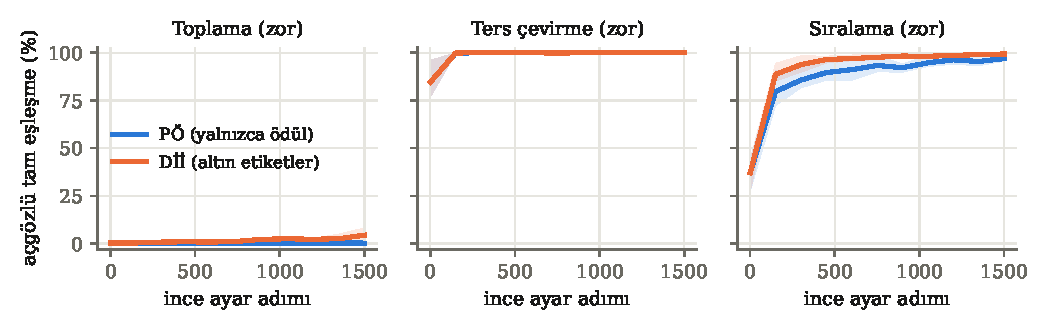
\includegraphics[width=0.92\textwidth]{fig_curves_tr.pdf}
\caption{2. aşama boyunca zor rejim doğruluğu: PÖ (ikili ödül, etiket yok) ve Dİİ (altın
etiketler). Çizgiler 3 seed'in ortalamasıdır; bantlar en küçük ve en büyük değeri kapsar.}
\label{fig:curves}
\end{figure*}

\begin{figure*}[t]
\centering
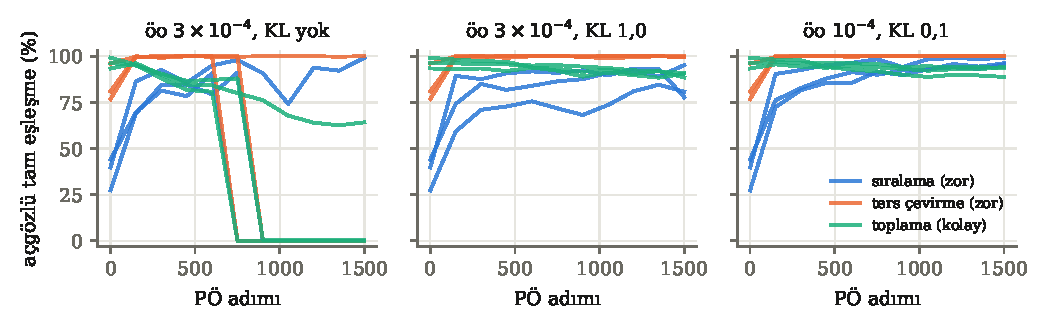
\includegraphics[width=0.92\textwidth]{fig_stability_tr.pdf}
\caption{Seed başına eğitim eğrileri (her seed ve ölçüt için bir çizgi). Solda: yüksek öğrenme
oranında KL çapası olmadan üç koşudan ikisi 600.--900. adımlar arasında tüm görevlerde çöküyor ve
toparlanmıyor. Ortada: güçlü bir çapa çökmeyi ortadan kaldırıyor ama sıralamadaki kazancı
yavaşlatıyor. Sağda: varsayılan yapılandırma.}
\label{fig:stability}
\end{figure*}

\section{Sonuçlar}
\paragraph{PÖ, kısmi yetkinliğin bulunduğu görevlerde açığın çoğunu kapatıyor.}
Tablo~\ref{tab:main} ve Şekil~\ref{fig:curves} ana karşılaştırmayı gösteriyor. Zor sıralamada PÖ
modeli \%37,1'den \%96,9'a taşıyor; Dİİ'de bu değer \%99,3. Zor ters çevirmede ikisi de \%100'e
ulaşıyor. Kazancın çoğu ilk 150 adımda geliyor. PÖ, sıralamada baştan sona Dİİ'nin biraz gerisinde
kalıyor; bu beklenen bir durum, çünkü bir etiket, örnek başına bir bitlik ödülden daha fazla bilgi
taşır.

\paragraph{PÖ, başlangıç başarı oranının sıfıra yakın olduğu yerde yardımcı olmuyor.}
Zor toplamada ön-eğitimli modeller test istemlerinin \%0,3'ünü doğru yanıtlıyor ve PÖ bunu
değiştirmiyor. İkili ödülle bir bölüm, ancak örneklenen cevap tam olarak doğruysa sıfırdan farklı
bir öğrenme sinyali üretir; dolayısıyla pekiştirilecek neredeyse hiçbir şey yoktur. Kısmen doğru
cevaplara puan veren biçimlendirilmiş ödül de bunu değiştirmedi (\%0,6). Cevabı gören Dİİ bile aynı
bütçede yalnızca \%4,4'e ulaşıyor; yani bu görev, sinyalden bağımsız olarak, bu boyuttaki ve bu
eğitim süresindeki model için zor. Deney, PÖ'nün soğuk başlangıcı aşamadığını gösteriyor; zorluğun
ne kadarının PÖ'ye özgü olduğunu ise göstermiyor.

\paragraph{PÖ, Dİİ'den daha az unuttu.}
İki yöntem de 2. aşamada kolay örnek görmüyor. Dİİ altında kolay toplama \%96,3'ten \%62,2'ye,
kolay sıralama \%97,6'dan \%91,4'e düşüyor. PÖ altında kolay toplama \%92,2'ye düşüyor, kolay
sıralama ise düşmüyor. KL çapası bunun küçük bir kısmını açıklıyor: çapa olmadan da PÖ kolay
toplamada \%89,7'yi koruyor. Nedeni sınamadık. Verilerle tutarlı bir açıklama şu: Dİİ, henüz
çözemediği ve kolay toplamayla aynı görev etiketini paylaşan zor toplamada büyük gradyanlar
uyguluyor; PÖ ise ödül neredeyse hep sıfır olduğu için orada neredeyse hiç gradyan almıyor.

\paragraph{Tek bir görevde eğitim diğerlerine zarar veriyor.}
Yalnızca zor sıralamayı ödüllendirmek onu \%99,1'e getiriyor, ancak zor ters çevirme \%84,6'dan
\%73,9'a, kolay toplama \%96,3'ten \%84,9'a düşüyor; üstelik KL çapası varken (bu koşuda çapa
yalnızca sıralama istemlerinde uygulanıyor). Çok görevli ödül bunu önledi.

\paragraph{Çökme ve KL çapası.}
Öğrenme oranı $3\times10^{-4}$ iken ve KL terimi yokken üç koşudan ikisi 600--750 adım boyunca
iyileşiyor, ardından tek bir değerlendirme aralığı içinde altı test kümesinin tümünde \%0'a
düşüyor ve toparlanmıyor (Şekil~\ref{fig:stability}, sol). Aynı başarısızlığın görüldüğü daha
önceki bir deneme koşusunda, çöken model dizi sonu simgesini üretmeyi bırakmış ve en büyük
uzunlukta dizgiler üretmişti. $\beta=1$ ile üç koşu da kararlı, ancak zor sıralama yalnızca
\%84,6'ya ulaşıyor. Öğrenme oranı $10^{-4}$ iken çapa olsun olmasın hiçbir koşu çökmedi; yani bu
düzenekte çapa, saldırgan bir adım büyüklüğüne karşı sigorta olarak önem taşıyor, varsayılan
yapılandırma için ise gerekli değildi.

\paragraph{Taban değer ve ödül biçimlendirme ölçülebilir bir fark yaratmadı.}
Taban değeri kaldırmak zor sıralamada \%99,5 verdi (taban değerle \%96,9); biçimlendirilmiş ödül
\%97,0 verdi. Üç seed ve 0,3--1,6 puanlık standart sapmalarla, taban değersiz varyantın 2,6
puanlık üstünlüğünü kanıtlanmış saymıyoruz; ancak taban değerin bir yarar sağlamadığı açık.
Negatif olmayan ikili ödülle ve taban değer olmadan güncelleme, modelin kendi doğru örnekleri
üzerinde bir olabilirlik adımıdır; başarı sık olduğunda bu düşük varyanslı bir sinyaldir.

\section{İlgili çalışmalar}
REINFORCE~\cite{williams1992}, türevlenemeyen ölçütleri eniyilemek için dizi üretimine, olabilirlikle
ön-eğitilmiş bir modelden başlanarak uygulanmış~\cite{ranzato2016}, taban değer olarak çoğu kez
modelin kendi açgözlü çıktısı kullanılmıştır~\cite{rennie2017}. PÖ sırasında ön-eğitimli modelden
sapmanın cezalandırılması dizi modelleri için Jaques ve ark.~\cite{jaques2017} tarafından
önerilmiştir ve büyük modellerin tercih temelli ayarında, genellikle PPO~\cite{schulman2017} ile
birlikte standarttır~\cite{ouyang2022}. Matematik ve akıl yürütme görevlerinde ölçekli, doğrulayıcı
ödüllü eğitim~\cite{shao2024,guo2025} çalışmalarında anlatılır. Aritmetik üzerinde eğitilen küçük
transformer'lar, öğrenme dinamiklerini incelemek için yaygın bir deney ortamıdır~\cite{lee2024}.
Katkımız yeni bir yöntem değil; bu tarifin yararlarının ve başarısızlık biçimlerinin seed'ler
üzerinde ölçülebildiği, asgari ve tümüyle yeniden üretilebilir bir düzenektir.

\section{Sınırlılıklar}
Model, görevler ve bütçeler çok küçüktür; buradaki hiçbir şey aynı etkilerin büyük ölçekte de
geçerli olduğunu göstermez. Tüm sonuçlar üç seed kullanır; bu, büyük etkileri (sıralamadaki kazanç,
unutma farkı, çökme) görmek için yeterli, birkaç puanla ayrışan ablasyonları sıralamak için
yetersizdir. Hiperparametreler seed 0 üzerinde küçük bir deneme taramasıyla seçilmiştir. Test
istemleri, eğitim istemleriyle aynı üreteçlerden, çakışmalar ayıklanmadan çekilmiştir; bu, zor
rejim için pek önem taşımaz (istem uzayı büyüktür), ancak kolay rejim sayılarının genellemeyi
değil, akılda tutmayı ölçtüğü anlamına gelir. Tek bir PÖ algoritmasını sınadık; PPO tarzı kırpma,
daha büyük yığınlar veya kolaydan zora bir müfredat, toplamadaki soğuk başlangıç sonucunu
değiştirebilir; bunları denemedik. Unutma farkı ve çökme için sunulan açıklamalar, deneylerin
sınamadığı hipotezlerdir.

\section{Sonuç}
344 bin parametreli bir dil modelinde, ikili doğrulayıcı ödülüyle çalışan yalın REINFORCE, modelin
zaten ara sıra çözebildiği görevlerde denetimli ince ayarın yararının neredeyse tamamını yakaladı,
eğitilmediği şeyleri daha az unuttu ve henüz hiç çözemediği bir görevde işe yaramadı. Ön-eğitimli
modele bağlanan bir KL çapası, yüksek öğrenme oranındaki ani çökmeye karşı korudu. Kod her şeyi
sıfırdan, tek bir işlemci çekirdeğinde koşu başına yaklaşık on dakikada eğitiyor; bu da düzeneği,
PÖ ile ince ayara ilişkin fikirleri GPU zamanı harcamadan önce sınamak için elverişli kılıyor.

\paragraph{Yeniden üretilebilirlik.} Tüm kod \texttt{tinyrl.py} (model, görevler, eğitim),
\texttt{run\_all.sh} (deney ızgarası) ve \texttt{analyze.py} (tablo ve şekiller) dosyalarındadır.
Tek işlemci çekirdeğinde duvar saati süresi: ön-eğitim yaklaşık 6, bir PÖ koşusu 10, bir Dİİ koşusu
4 dakika.

\begin{thebibliography}{9}
\small
\bibitem{williams1992} R.~J. Williams. Simple statistical gradient-following algorithms for
connectionist reinforcement learning. \emph{Machine Learning}, 8(3--4):229--256, 1992.
\bibitem{vaswani2017} A.~Vaswani ve ark. Attention is all you need. \emph{NeurIPS}, 2017.
\bibitem{ranzato2016} M.~Ranzato, S.~Chopra, M.~Auli, W.~Zaremba. Sequence level training with
recurrent neural networks. \emph{ICLR}, 2016.
\bibitem{rennie2017} S.~Rennie ve ark. Self-critical sequence training for image captioning.
\emph{CVPR}, 2017.
\bibitem{jaques2017} N.~Jaques ve ark. Sequence Tutor: Conservative fine-tuning of sequence
generation models with KL-control. \emph{ICML}, 2017.
\bibitem{schulman2017} J.~Schulman ve ark. Proximal policy optimization algorithms.
\emph{arXiv:1707.06347}, 2017.
\bibitem{ouyang2022} L.~Ouyang ve ark. Training language models to follow instructions with human
feedback. \emph{NeurIPS}, 2022.
\bibitem{shao2024} Z.~Shao ve ark. DeepSeekMath: Pushing the limits of mathematical reasoning in
open language models. \emph{arXiv:2402.03300}, 2024.
\bibitem{guo2025} D.~Guo ve ark. DeepSeek-R1: Incentivizing reasoning capability in LLMs via
reinforcement learning. \emph{Nature}, 645:633--638, 2025.
\bibitem{lee2024} N.~Lee ve ark. Teaching arithmetic to small transformers. \emph{ICLR}, 2024.
\end{thebibliography}
\end{document}
